%\begin{appendices}

\appendix
%\chapter*{ANEXOS}% If \appendix doesn't insert a \chapter
%\addcontentsline{toc}{chapter}{ANEXOS}% Print Appendix in ToC
\setcounter{section}{0}% Reset numbering for sections
\renewcommand{\thesection}{\Alph{section}}% Adjust section printing (from here onward)
	
	\section{Árbol de Problemas}
	%\chapter*{Árbol de Problemas}
	%\addcontentsline{toc}{section}{Árbol de Problemas}
	%\renewcommand{\thechapter}{A}
	\label{anexo1}
	\begin{figure}[h]
		\begin{center}
			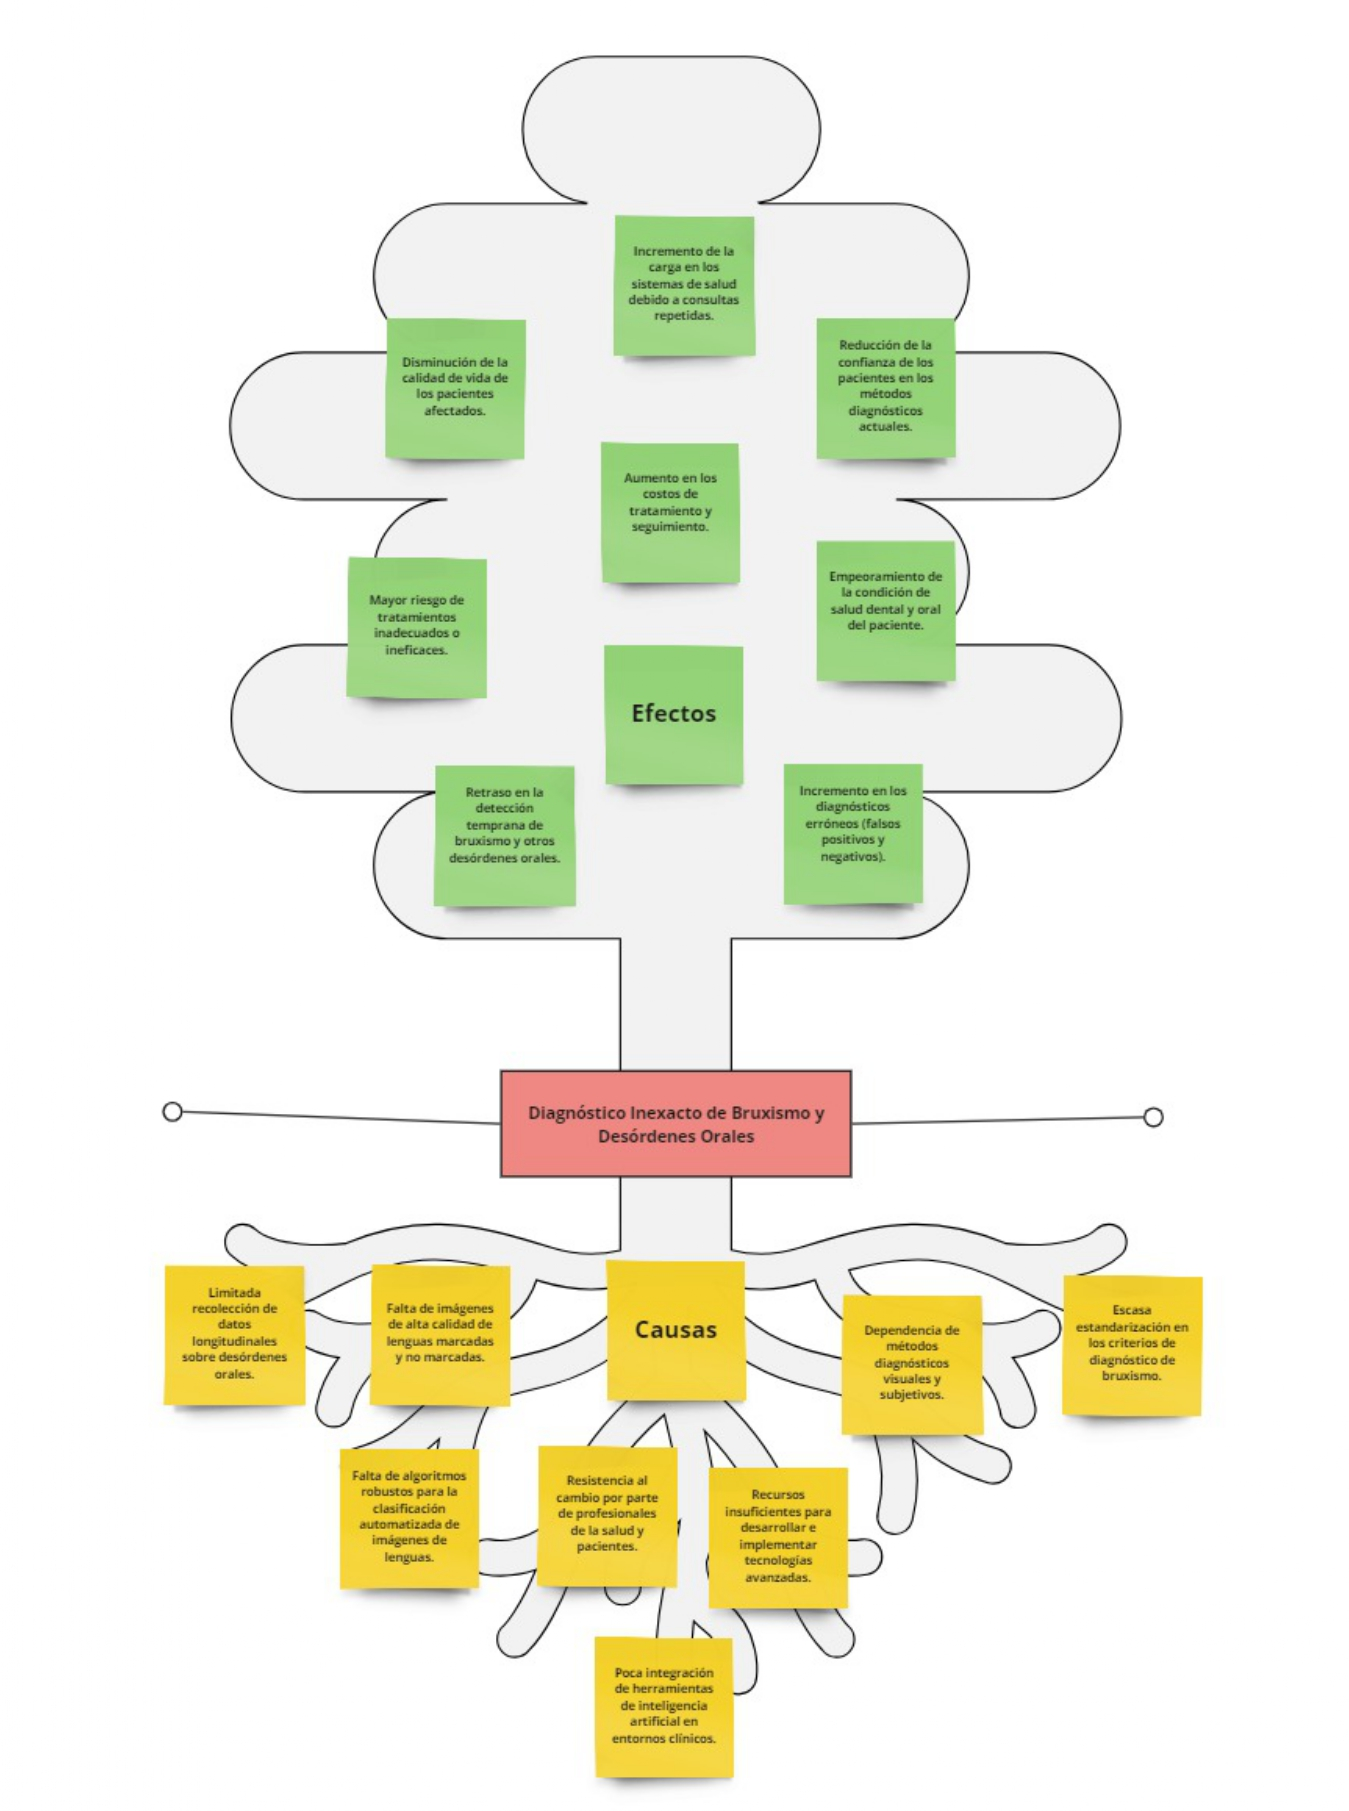
\includegraphics[width=0.85\textwidth]{anexos/arbol_problematica.jpg}
			%\caption{Fuente: Elaboración propia}
		\end{center}
	\end{figure}
	\clearpage

	\section{Matriz de contingencia}
\begin{table}[H]
    \caption{Problema, objetivos y variables de la investigación.}
    \centering
    \renewcommand{\arraystretch}{1.5} % Aumenta el espacio entre filas
    \setlength{\tabcolsep}{10pt} % Ajusta el espacio entre columnas
    \begin{tabular}{|p{4cm}|p{5cm}|p{6cm}|}
        \hline
        \textbf{Problema} & \textbf{Objetivo} & \textbf{Variables} \\ \hline
        \textbf{Principal:} ¿Cómo puede un sistema automatizado, basado en técnicas de aprendizaje profundo, realizar un prediagnóstico efectivo del bruxismo en niños? 
        & Desarrollar y validar un sistema automatizado basado en técnicas de aprendizaje profundo para el prediagnóstico de bruxismo en niños. 
        & 
        \textbf{Dependiente:} Precisión del prediagnóstico de bruxismo. \\
        & & \textbf{Independiente:} Técnicas de procesamiento de imágenes, patrones visuales. \\ \hline
        \textbf{Específicos:} 
        \begin{itemize}
            \item ¿Cuáles son los patrones visuales en imágenes de la lengua que están asociados con el bruxismo? 
            \item ¿Qué técnicas de procesamiento son más efectivas para identificar signos de bruxismo?
        \end{itemize} 
        & 
        \begin{itemize}
            \item Identificar patrones visuales en imágenes de la lengua indicativos de bruxismo infantil.
            \item Evaluar técnicas de procesamiento y extracción de características.
        \end{itemize} 
        & 
        \textbf{Dependiente:} Detección temprana de bruxismo. \\
        & & \textbf{Independiente:} Redes neuronales convolucionales (CNN), imágenes de la lengua. \\ \hline
    \end{tabular}
\end{table}

	
	\clearpage